\documentclass{beamer}

\usetheme{metropolis}

\usepackage[ngerman]{babel}
\usepackage[autostyle=true,german=quotes]{csquotes}
\usepackage[linewidth=1pt]{mdframed}
\usepackage{hyperref}
\usepackage{makecell}
\usepackage{pifont}
\usepackage{tikz}
\usetikzlibrary{positioning, calc, arrows, fit, decorations.pathreplacing, shapes, shapes.multipart, snakes}
\usepackage{verbatim}
\usepackage{textcomp}
\usepackage{centernot}
\usepackage{tabularx}
\usepackage{ulem}
%\usepackage{pdfpages}

\batchmode

\hypersetup{
	colorlinks,
	urlcolor=blue,
	linkcolor=black % for ToC
}
\newenvironment{qaa}[1]{
	#1

	\begin{mdframed}
		\small
}{
	\end{mdframed}
}

\newcommand{\true}{\ding{51}}
\newcommand{\false}{\ding{55}}
\newcommand{\code}[1]{
	\begin{mdframed}
		\verbatiminput{#1}
	\end{mdframed}
}


\title{Tutorium 07: Prolog, Typinferenz}
% \subtitle{}
\author{Paul Brinkmeier}
\institute{Tutorium Programmierparadigmen am KIT}
\date{15. Dezember 2020}

\begin{document}

\begin{frame}
	\titlepage
\end{frame}

\section{Heutiges Programm}

\begin{frame}{Programm}
	\begin{itemize}
                \item Typinferenz
		\item Aufgaben zu Prolog
	\end{itemize}
\end{frame}

\section{Typinferenz}

\subsection{Unifikation}

% https://tex.stackexchange.com/questions/57441/how-to-include-existing-pdf-slides-into-my-beamer-presentation
{
\setbeamercolor{background canvas}{bg=}
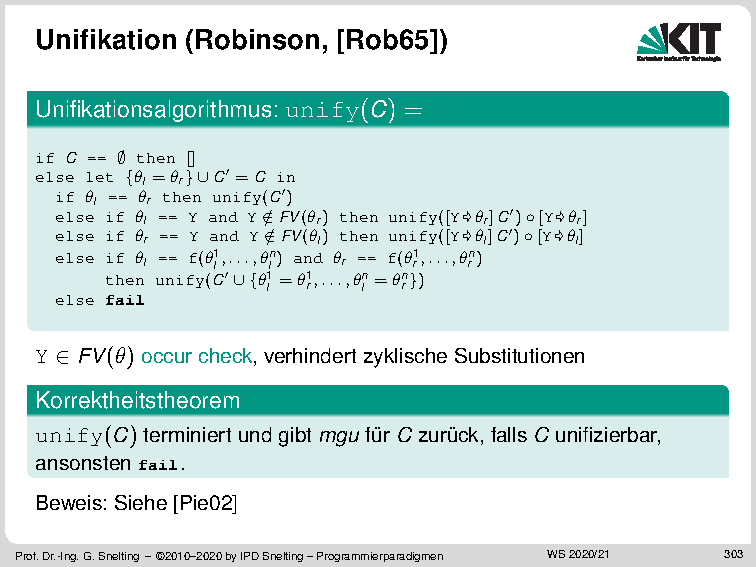
\includepdf{robinson.pdf}
}

\begin{frame}{Prolog-Unifikation}
	Unifiziert:

	\begin{itemize}
		\item \texttt{A = x}
		\item \texttt{B = f(x)}
		\item \texttt{C = g(C)}
		\item \texttt{f(x, A, z) = f(x, y, B)}
                \item \texttt{func(A, B, z) = func(x, y, A)}
		\item \texttt{g(x, A, z) = f(x, A, A)}
		\item \texttt{f(g(z)) = f(D)}
	\end{itemize}

	Ergebnis: Entweder \textbf{fail} oder ein Unifikator.
\end{frame}

\begin{frame}{Cheatsheet: Lambda-Kalkül/Basics}
  \begin{itemize}
    \item Terme $t$: Variable ($x$), Funktion ($\lambda x . t$), Anwendung ($t \; t$)
    \item \emph{$\alpha$-Äquivalenz}: Gleiche Struktur
    \item \emph{$\eta$-Äquivalenz}: Unterversorgung
    \item \emph{Freie Variablen}, \emph{Substitution}, \emph{RedEx}
    \item \emph{$\beta$-Reduktion}: \\
          $(\lambda{}p.b)$ $t \Rightarrow b\left[p\rightarrow{}t\right]$
  \end{itemize}
\end{frame}

\subsection{Typinferenz}

\begin{frame}{Cheatsheet: Typisierter Lambda-Kalkül}
  \begin{mathpar}
    \inferrule{
      \Gamma{}(t) = \tau
    }{
      \Gamma \vdash t : \tau
    } \textrm{\textsc{Var}}
    \and
    \inferrule{
      \Gamma \vdash f : \phi \to \alpha \\
      \Gamma \vdash x : \phi
    }{
      \Gamma \vdash \app{f}{x} : \alpha
    } \textrm{\textsc{App}}
    \and
    \inferrule{
      \Gamma{}, p : \pi \vdash b : \rho
    }{
      \Gamma \vdash \lam{p}{b} : \pi \to \rho
    } \textrm{\textsc{Abs}}
  \end{mathpar}

  \begin{itemize}
    \item Typvariablen: $\tau$, $\alpha$, $\pi$, $\rho$
    \item Funktionstypen: $\tau_1 \to \tau_2$, rechtsassoziativ
    \item (Weitere Typen: Listen, Tupel, etc.)
    \item \emph{Typisierungsregeln sind eindeutig}: Eine Regel pro Termform
  \end{itemize}
\end{frame}

\begin{frame}{(Allgemeine) Typisierungsregel für Variablen}
	\begin{itemize}
		\item \tikz[baseline, remember picture]{\node [fill=green!20,draw] (varRetL) {\enquote{Der Typkontext $\Gamma$ enthält einen Typ $\tau$ für $t$.}};}
	\end{itemize}

	\begin{mathpar}
		\inferrule{
			\tikz[baseline, remember picture]{\node[fill=green!20,draw] (varRet) {$\Gamma{}(t) = \tau$};}
		}{
			\tikz[baseline, remember picture]{\node[fill=blue!20,draw] (varShow) {
				$\Gamma \vdash t : \tau$
			};}
		} \textrm{\textsc{Var}}
	\end{mathpar}

	\begin{itemize}
		\item Daraus folgt:
		\item \tikz[baseline, remember picture]{\node [fill=blue!20,draw] (varShowL) {\enquote{Variable $t$ hat im Kontext $\Gamma$ den Typ $\tau$.}};}
	\end{itemize}

	\tikz[overlay, remember picture]{
		\draw[->] (varShowL) edge [bend left] (varShow);
		\draw[->] (varRetL) edge [bend right] (varRet);
	}
\end{frame}

\newcommand{\tikzmark}[3]{\tikz[baseline, remember picture]{
	\node[fill=#1,draw] (#2) {#3};
}}

\begin{frame}{Typisierungsregel für Funktionsanwendungen}
	\begin{itemize}
		\item \tikzmark{green!20}{fTypeL}{\enquote{$f$ ist im Kontext $\Gamma$ eine Funktion, die $\phi$s auf $\alpha$s abbildet.}}
		\item \tikzmark{red!20}{aTypeL}{\enquote{$x$ ist im Kontext $\Gamma$ ein Term des Typs $\phi$.}}
	\end{itemize}
	\begin{mathpar}
		\inferrule{
			\tikzmark{green!20}{fType}{$\Gamma \vdash f : \phi \to \alpha$} \\
			\tikzmark{red!20}{aType}{$\Gamma \vdash x : \phi$}
		}{
			\tikzmark{blue!20}{eType}{$\Gamma \vdash \app{f}{x} : \alpha$}
                } \textrm{\textsc{App}}
	\end{mathpar}

	\begin{itemize}
		\item Daraus folgt:
		\item \tikzmark{blue!20}{eTypeL}{\enquote{$x$ eingesetzt in $f$ ergibt einen Term des Typs $\alpha$.}}
	\end{itemize}

	\tikz[overlay, remember picture]{
		\draw[->] (fTypeL) edge [bend right] (fType);
		\draw[->] (aTypeL) edge [bend left] (aType);
		\draw[->] (eTypeL) edge [bend left] (eType);
	}
\end{frame}

\begin{frame}{Typisierungsregel für Lambdas}
	\begin{itemize}
		\item \tikzmark{green!20}{contextL}{\enquote{Unter Einfügung des Typs $\pi$ von $p$ in den Kontext...}}
		\item \tikzmark{red!20}{bodyTypeL}{\enquote{... ist $b$ als Funktion von $p$ typisierbar.}}
	\end{itemize}

	\begin{mathpar}
		\inferrule{
			\tikzmark{green!20}{context}{$\Gamma{}, p : \pi$} \\
			\tikzmark{red!20}{bodyType}{$\vdash b : \rho$}
		}{
			\tikzmark{blue!20}{absType}{$\Gamma \vdash \lam{p}{b} : \pi \to \rho$}
                } \textrm{\textsc{Abs}}
	\end{mathpar}

	\begin{itemize}
		\item Daraus folgt:
		\item \tikzmark{blue!20}{absTypeL}{\enquote{$\lam{p}{b}$ ist eine Funktion, die $\pi$s auf $\rho$s abbildet}}
	\end{itemize}

	\tikz[overlay, remember picture]{
		\draw[->] (bodyTypeL) edge [bend left] (bodyType);
		\draw[->] (contextL) edge [bend right] (context);
		\draw[->] (absTypeL) edge [bend left] (absType);
	}
\end{frame}

\begin{frame}{Typinferenz}
	Vorgehensweise zur Typinferenz:
	\begin{itemize}
		\item Stelle Typherleitungsbaum auf
		\begin{itemize}
			\item In jedem Schritt werden neue Typvariablen $\alpha_i$ angelegt
			\item Statt die Typen direkt im Baum einzutragen, werden Gleichungen in einem Constraint-System eingetragen
		\end{itemize}
		\item Unifiziere Constraint-System zu einem Unifikator
		\begin{itemize}
			\item Robinson-Algorithmus, im Grunde wie bei Prolog
                        \item I.d.R.: Allgemeinster Unifikator (findet man per Robinson)
		\end{itemize}
	\end{itemize}
\end{frame}

{
\setbeamercolor{background canvas}{bg=}
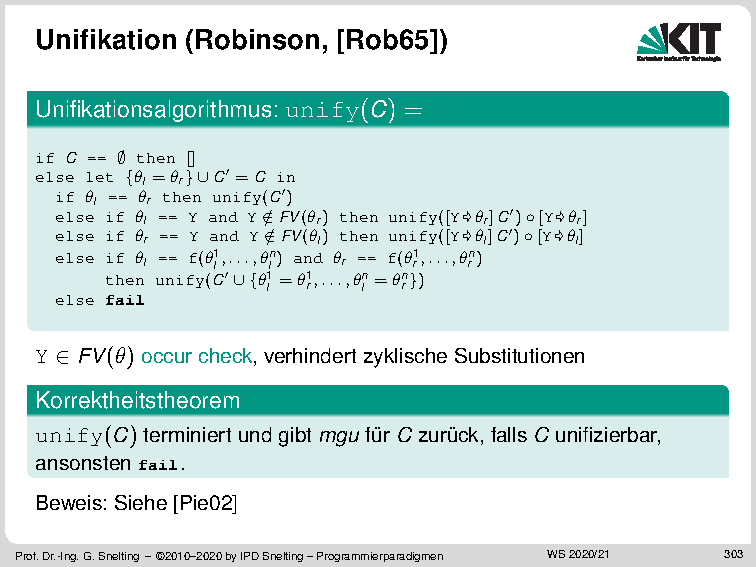
\includepdf{robinson.pdf}
}

{
\setbeamercolor{background canvas}{bg=}
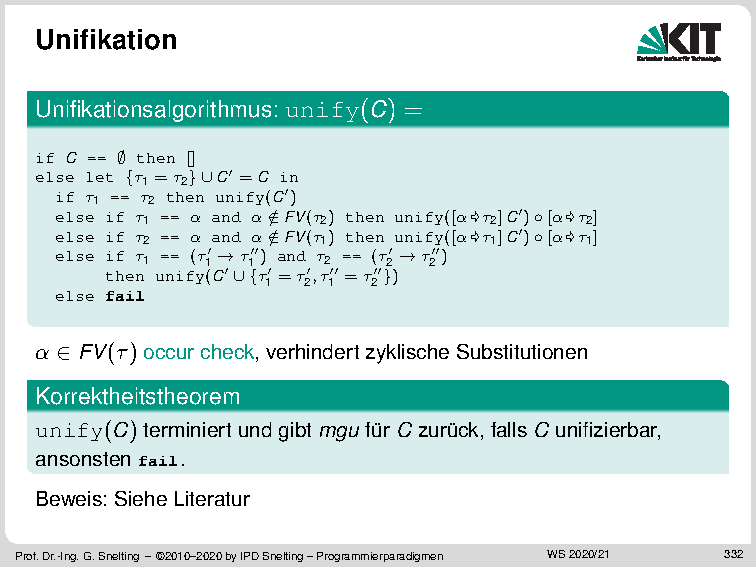
\includepdf{robinson2.pdf}
}

\begin{frame}{Unifikation für Typinferenz}
  \emph{Typen kann man auch als Funktoren darstellen}:

  \begin{align*}
    \tau_1 \to \tau_2   && \equiv && \texttt{func}(\tau_1, \tau_2) \\
    \left[ \tau \right] && \equiv && \texttt{list}(\tau) \\
                        && \text{etc.}
  \end{align*}
\end{frame}

\begin{frame}{Typinferenz: Übungsaufgaben}
	\only<1>{
	\begin{mathpar}
		\inferrule{
			...
		}{
                  f : \textrm{int} \to \beta \vdash \lam{x}{\app{f}{x}} : \alpha_1
                } \textrm{\textsc{Abs}}
	\end{mathpar}

	\begin{itemize}
		\item \enquote{Finde den allgemeinsten Typen $\alpha_1$ von $\lam{x}{\app{f}{x}}$}
	\end{itemize}
	}

	\only<2>{
	\begin{mathpar}
		\inferrule{
			...
		}{
                  \vdash \lam{f}{\lam{x}{\app{(\app{f}{x})}{x}}} : \alpha_1
                } \textrm{\textsc{Abs}}
	\end{mathpar}

	\begin{itemize}
          \item \enquote{Finde den allgemeinsten Typen $\alpha_1$ von $\lam{f}{\lam{x}{\app{(\app{f}{x})}{x}}}$}
	\end{itemize}
	}


	Erinnerung:

	\begin{itemize}
		\item Baum mit durchnummerierten $\alpha_i$ aufstellen
		\item Constraints sammeln:
	\end{itemize}

	\begin{columns}
		\scriptsize
		\begin{column}{0.3\textwidth}
                  \begin{mathpar}
    \inferrule{
      \Gamma{}(t) = \alpha_j
    }{
      \Gamma \vdash t : \alpha_i
    } \textrm{\textsc{Var}}
                  \end{mathpar}

                  \center
                        Constraint:\\$\{ \alpha_i = \alpha_j \}$
		\end{column}
		\begin{column}{0.3\textwidth}
                  \begin{mathpar}
    \inferrule{
      \Gamma \vdash f : \alpha_j \\
      \Gamma \vdash x : \alpha_k
    }{
      \Gamma \vdash \app{f}{x} : \alpha_i
    } \textrm{\textsc{App}}
                  \end{mathpar}
\center
			Constraint:\\$\{ \alpha_j = \alpha_k \to \alpha_i \}$
		\end{column}
		\begin{column}{0.3\textwidth}
                  \begin{mathpar}
    \inferrule{
      \Gamma{}, p : \alpha_j \vdash b : \alpha_k
    }{
      \Gamma \vdash \lam{p}{b} : \alpha_i
    } \textrm{\textsc{Abs}}
                  \end{mathpar}
                        \center
			Constraint:\\$\{ \alpha_i = \alpha_j \to \alpha_k \}$
		\end{column}
	\end{columns}

	\begin{itemize}
		\item Constraint-System auflösen
	\end{itemize}
\end{frame}

\section{Prolog}

\subsection{Cheatsheet}

\begin{frame}{Cheatsheet: Prolog}
  \begin{itemize}
    \item Terme:
    \begin{itemize}
      \item Variablen: \texttt{Var}, \texttt{X}, \texttt{X2}
      \item Funktoren/Atome: \texttt{f(a, b, c)}, \texttt{app(f, x)}, \texttt{main}
      \item Arithmetische Ausdrücke: \texttt{17 + 25}, \texttt{6 * 7}
    \end{itemize}
    \item Regeln: \texttt{rule(P1, ..., PN) :- Goal1, ..., GoalM.}
    \item Ziele:
    \begin{itemize}
      \item Funktor: \texttt{member(X, [1,2,3])}
      \item Unifikation: \texttt{X = Y}
      \item Arithmetik: \texttt{N is M + 1}
      \item Verneinung: \texttt{not(G)}
      \item Arithmetischer Vergleich: \texttt{X =:= Y}, \texttt{X =\textbackslash= Y}, etc.
      \item Cut: \texttt{!}
    \end{itemize}
    \item Konzepte: \emph{Unifikation}, \emph{Resolution}
  \end{itemize}
\end{frame}

\begin{frame}{Prolog --- Regelsysteme als Programmiersprache}
  \code{../demos/grandparents.pl}

  \vfill

  \only<1>{
    \texttt{?- grandparent(inge, kunibert).} $\leadsto$ \texttt{yes.}
  }

  \only<2>{
    \begin{mathpar}
      \inferrule{
        \inferrule{
          \inferrule{ }{\text{\texttt{mother(inge, emil)}}}
        }{
          \text{\texttt{parent(inge, emil)}}
        } \\
        \inferrule{
          \inferrule{ }{\text{\texttt{father(emil, kunibert)}}}
        }{
          \text{\texttt{parent(emil, kunibert)}}
        }
      }{
        \text{\texttt{grandparent(inge, kunibert)}}
      }
    \end{mathpar}
  }
\end{frame}

\subsection{Bettenverteilung}

\begin{frame}{Schlafplätze im Gefängnis}
	\begin{figure}
		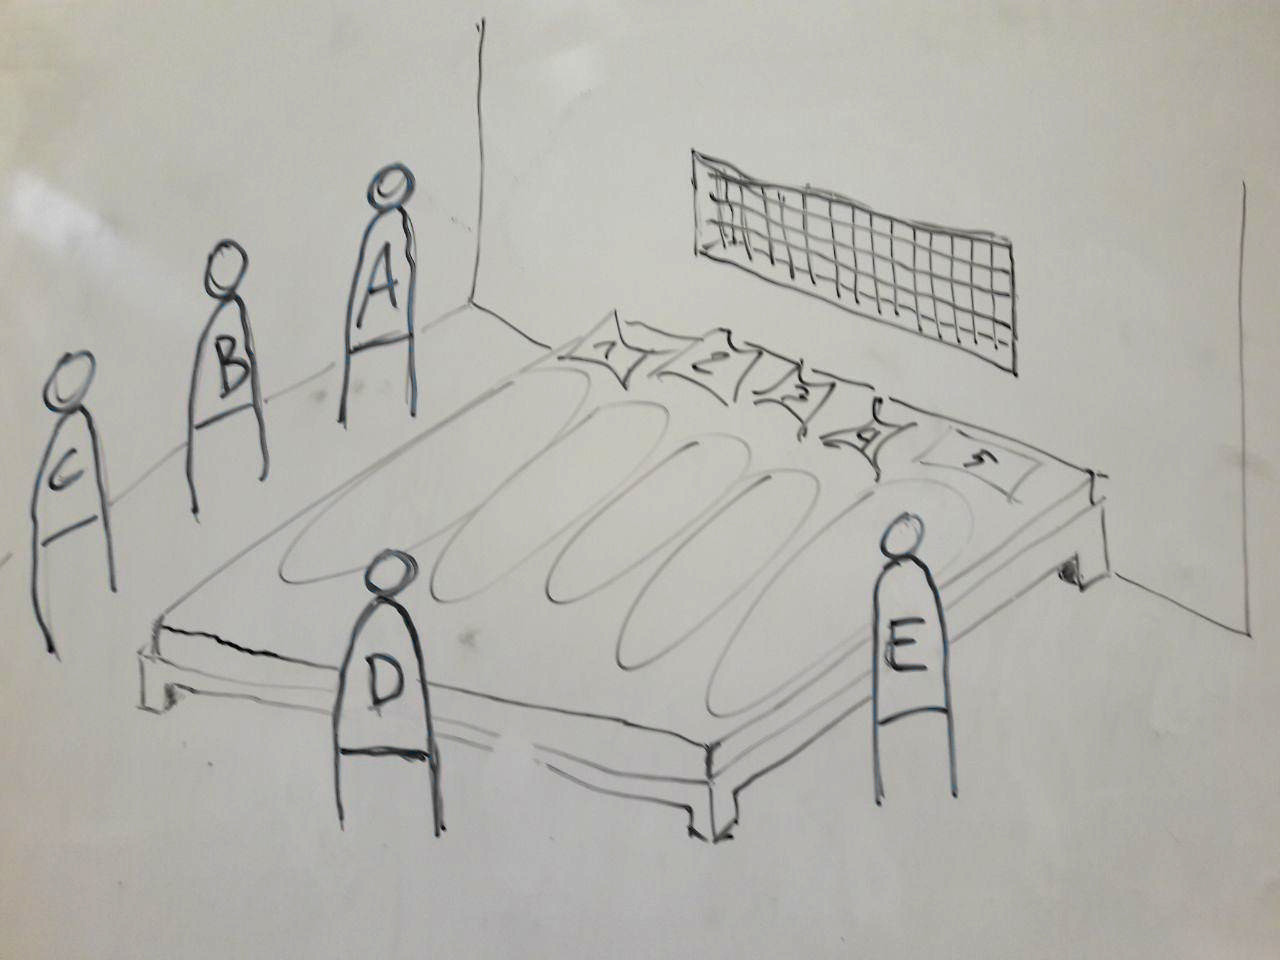
\includegraphics[width=0.8\textwidth]{images/bett}
	\end{figure}
\end{frame}

\begin{frame}{Dinesman's multiple-dwelling problem}
	Bob kommt nun ins Gefängnis.
	Aaron, Bob, Connor, David und Edison müssen sich zu fünft ein sehr breites Bett teilen.

	\begin{itemize}
		\item Aaron will nicht am rechten Ende liegen
		\item Bob will nicht am linken Ende liegen
		\item Connor will an keinem der beiden Enden liegen
		\item David will weiter rechts liegen als Bob
		\item Connor schnarcht sehr laut;\\Bob und Edison sind sehr geräuschempfindlich
		\begin{itemize}
			\item $\leadsto$ Bob will nicht direkt neben Connor liegen
			\item $\leadsto$ Edison will nicht direkt neben Connor liegen
		\end{itemize}
	\end{itemize}

	Wie können die 5 Schlafplätze verteilt werden?
\end{frame}

\begin{frame}{Schlafplätze im Gefängnis}
	\code{../demos/schlafplaetze.pl}

	\begin{itemize}
		\item Fügt weitere benötigte Tests ein
		\item Implementiert:
		\begin{itemize}
			\item \texttt{distinct/1} prüft Listenelemente auf paarweise Ungleichheit
			\item \texttt{adjacent/2} prüft, ob $|A - B| = 1$
		\end{itemize}
	\end{itemize}
\end{frame}

% ansatz: multipleDwelling(B, C, F, M, S) :- ....
% distinct/1
% adjacent/2

\subsection{Putzdienst}

\begin{frame}{Putzdienst}
	\begin{figure}
		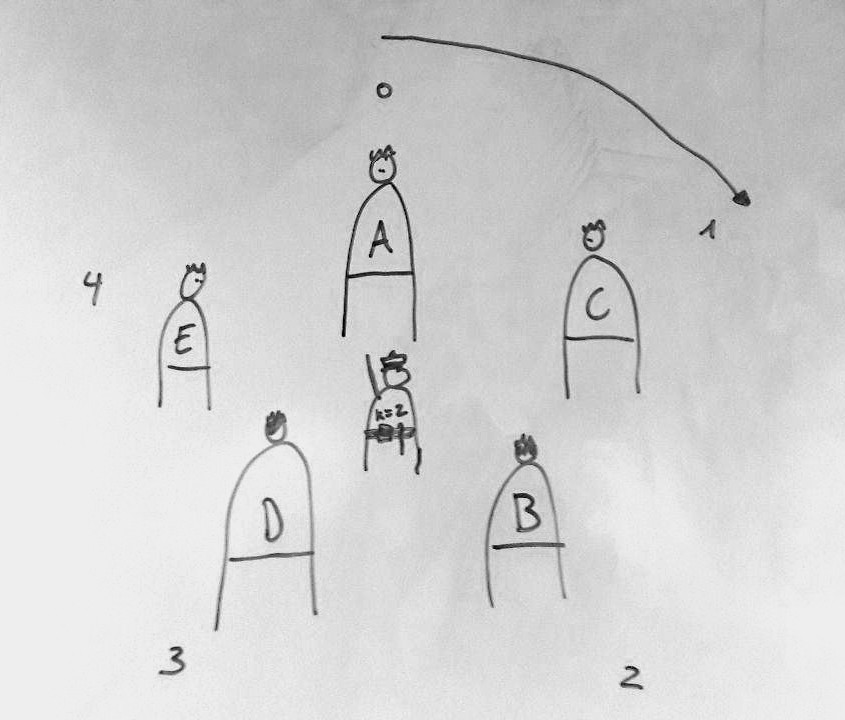
\includegraphics[width=0.7\textwidth]{images/putzdienst}
	\end{figure}
\end{frame}

\begin{frame}{Putzdienst}
	\begin{itemize}
		\item Aaron, Bob, Connor, David und Edison sollen 4 Einheiten Putzdienst übernehmen
		\item Da sie sich nicht einigen können, wer aussetzen darf, wendet ein Wärter folgendes Vorgehen an:
		\begin{itemize}
			\item Die fünf werden im Kreis aufgestellt
			\item Der Wärter stellt sich in die Mitte
			\item Beginnend bei 12 Uhr dreht er sich im Uhrzeigersinn und teilt jeden $k$-ten (bspw. $k = 2$) Insassen zum Putzdienst ein
			\begin{itemize}
				\item D.h. es werden immer $k - 1$ Insassen übersprungen
			\end{itemize}
		\end{itemize}
	\end{itemize}

	An welcher Stelle muss Bob stehen, um nicht putzen zu müssen?\\
	\pause
	An welcher Stelle muss Bob bei 41 Insassen und $k = 3$ stehen?
\end{frame}

\begin{frame}{Putzdienst}
	\code{../demos/putzdienst.pl}

	\begin{itemize}
		\item Weitere Fälle für \texttt{helper/4}:
		\begin{itemize}
			\item \texttt{C = 0} $\leadsto$ Element entfernen
			\item Ansonsten: Element hinten wieder anhängen
		\end{itemize}
	\end{itemize}
\end{frame}

\subsection{Quellen}

\begin{frame}{Quellen der Aufgaben}
	Zum Nachlesen und Vergleichen mit Lösungen in anderen Programmiersprachen:
	\begin{itemize}
		\item WG --- \href{https://rosettacode.org/wiki/Department_Numbers}{Rosetta Code: Department Numbers}
		\item Detektiv --- \href{https://github.com/Anniepoo/prolog-examples/blob/master/newdetective.pl}{github.com/Anniepoo/prolog-examples}
		\item Schlafplätze --- SICP, S. 418
		\item Putzdienst --- \href{https://rosettacode.org/wiki/Josephus_problem}{Rosetta Code: Josephus problem}
	\end{itemize}
\end{frame}

% quellen:
% multiple dwelling: SICP S. 418
% detective: https://github.com/Anniepoo/prolog-examples/blob/master/newdetective.pl
% department numbers: https://rosettacode.org/wiki/Department_Numbers
% josephus problem: https://rosettacode.org/wiki/Josephus_problem#Python

\section{Schöne Ferien!}

\begin{frame}{Schöne Ferien!}

  \begin{itemize}
    \item Nach dem Ferien: Mehr Typinferenz, Reussner-Teil
    \item Aktueller Klausurtermin:\\
          09.04.2021, 17:00, Zelt auf dem Forum
  \end{itemize}

  \vfill

  Bleibt gesund, feiert schön und einen guten Rutsch!
\end{frame}

\end{document}
